% 图 2.10 居里定律：(a) chi ~ 1/T (b) 1/chi 对 T 直线 (c) chi*T 为常数
\documentclass[tikz,border=5pt]{standalone}
\usetikzlibrary{arrows.meta}
\usepackage{amsmath}
\usepackage{bm}
\usepackage{fontspec}
\setmainfont{Times New Roman}
\begin{document}
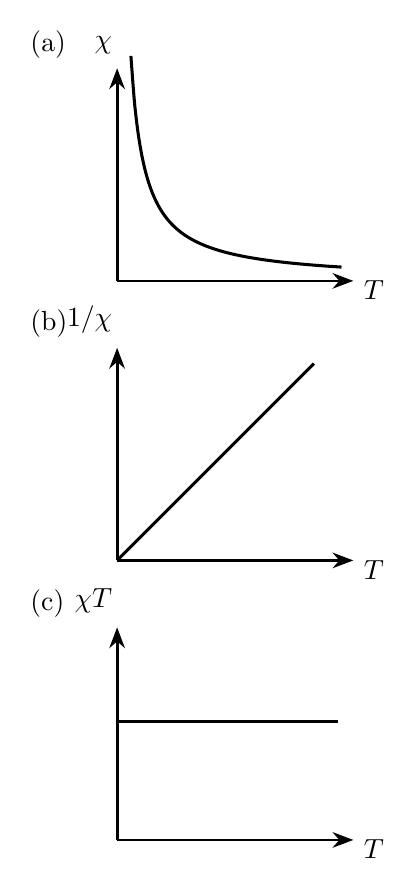
\begin{tikzpicture}[line width=0.8pt,>=Stealth]
% ---------- (a) ----------
\begin{scope}[shift={(0.9,0)}]
\node[anchor=south west,inner sep=1pt] at (-1.15,2.78) {(a)};
\draw[->,line width=1.0pt] (0,0) -- (0,2.7);
\draw[->,line width=1.0pt] (0,0) -- (3.0,0);
\node[anchor=south east,inner sep=2pt] at (0.02,2.8) {$\chi$};
\node[anchor=west,inner sep=2pt] at (3.05,-0.12) {$T$};
\draw[very thick,line width=1.1pt] plot[domain=0.175:2.85,samples=60,smooth]
  ({\x},{0.5/\x});
\end{scope}
% ---------- (b) ----------
\begin{scope}[shift={(0.9,-3.55)}]
\node[anchor=south west,inner sep=1pt] at (-1.15,2.78) {(b)};
\draw[->,line width=1.0pt] (0,0) -- (0,2.7);
\draw[->,line width=1.0pt] (0,0) -- (3.0,0);
\node[anchor=south east,inner sep=2pt] at (0.02,2.8) {$1/\chi$};
\node[anchor=west,inner sep=2pt] at (3.05,-0.12) {$T$};
\draw[very thick,line width=1.1pt] (0,0) -- (2.5,2.5);
\end{scope}
% ---------- (c) ----------
\begin{scope}[shift={(0.9,-7.1)}]
\node[anchor=south west,inner sep=1pt] at (-1.15,2.78) {(c)};
\draw[->,line width=1.0pt] (0,0) -- (0,2.7);
\draw[->,line width=1.0pt] (0,0) -- (3.0,0);
\node[anchor=south east,inner sep=2pt] at (0.02,2.8) {$\chi T$};
\node[anchor=west,inner sep=2pt] at (3.05,-0.12) {$T$};
\draw[very thick,line width=1.1pt] (0,1.5) -- (2.8,1.5);
\end{scope}
\end{tikzpicture}
\end{document}
